\documentclass{article}\usepackage[]{graphicx}\usepackage[]{color}
%% maxwidth is the original width if it is less than linewidth
%% otherwise use linewidth (to make sure the graphics do not exceed the margin)
\makeatletter
\def\maxwidth{ %
  \ifdim\Gin@nat@width>\linewidth
    \linewidth
  \else
    \Gin@nat@width
  \fi
}
\makeatother

\definecolor{fgcolor}{rgb}{0.345, 0.345, 0.345}
\newcommand{\hlnum}[1]{\textcolor[rgb]{0.686,0.059,0.569}{#1}}%
\newcommand{\hlstr}[1]{\textcolor[rgb]{0.192,0.494,0.8}{#1}}%
\newcommand{\hlcom}[1]{\textcolor[rgb]{0.678,0.584,0.686}{\textit{#1}}}%
\newcommand{\hlopt}[1]{\textcolor[rgb]{0,0,0}{#1}}%
\newcommand{\hlstd}[1]{\textcolor[rgb]{0.345,0.345,0.345}{#1}}%
\newcommand{\hlkwa}[1]{\textcolor[rgb]{0.161,0.373,0.58}{\textbf{#1}}}%
\newcommand{\hlkwb}[1]{\textcolor[rgb]{0.69,0.353,0.396}{#1}}%
\newcommand{\hlkwc}[1]{\textcolor[rgb]{0.333,0.667,0.333}{#1}}%
\newcommand{\hlkwd}[1]{\textcolor[rgb]{0.737,0.353,0.396}{\textbf{#1}}}%

\usepackage{framed}
\makeatletter
\newenvironment{kframe}{%
 \def\at@end@of@kframe{}%
 \ifinner\ifhmode%
  \def\at@end@of@kframe{\end{minipage}}%
  \begin{minipage}{\columnwidth}%
 \fi\fi%
 \def\FrameCommand##1{\hskip\@totalleftmargin \hskip-\fboxsep
 \colorbox{shadecolor}{##1}\hskip-\fboxsep
     % There is no \\@totalrightmargin, so:
     \hskip-\linewidth \hskip-\@totalleftmargin \hskip\columnwidth}%
 \MakeFramed {\advance\hsize-\width
   \@totalleftmargin\z@ \linewidth\hsize
   \@setminipage}}%
 {\par\unskip\endMakeFramed%
 \at@end@of@kframe}
\makeatother

\definecolor{shadecolor}{rgb}{.97, .97, .97}
\definecolor{messagecolor}{rgb}{0, 0, 0}
\definecolor{warningcolor}{rgb}{1, 0, 1}
\definecolor{errorcolor}{rgb}{1, 0, 0}
\newenvironment{knitrout}{}{} % an empty environment to be redefined in TeX

\usepackage{alltt}
%\VignetteIndexEntry{Principal Component of Explained Variance}
%\VignetteEngine{knitr::latex}
\usepackage[utf8]{inputenc}
\IfFileExists{upquote.sty}{\usepackage{upquote}}{}
\begin{document}

\begin{knitrout}
\definecolor{shadecolor}{rgb}{0.969, 0.969, 0.969}\color{fgcolor}\begin{kframe}
\begin{alltt}
\hlkwd{library}\hlstd{(pcev)}
\end{alltt}


{\ttfamily\noindent\itshape\color{messagecolor}{\#\# PCEV: Principal components of explained variance}}\begin{alltt}
\hlkwd{data}\hlstd{(methylation)}
\hlkwd{data}\hlstd{(pheno)}
\hlkwd{data}\hlstd{(position)}
\end{alltt}
\end{kframe}
\end{knitrout}


\begin{knitrout}
\definecolor{shadecolor}{rgb}{0.969, 0.969, 0.969}\color{fgcolor}\begin{kframe}
\begin{alltt}
\hlcom{# Compute nominal pvalues}
\hlstd{fit} \hlkwb{<-} \hlkwd{lm}\hlstd{(methylation} \hlopt{~} \hlstd{pheno)}
\hlstd{pval} \hlkwb{<-} \hlkwd{vapply}\hlstd{(}\hlkwd{summary}\hlstd{(fit),} \hlkwa{function}\hlstd{(}\hlkwc{sum}\hlstd{) \{}
  \hlstd{pvalue} \hlkwb{<-} \hlstd{sum}\hlopt{$}\hlstd{coef[}\hlnum{2}\hlstd{,}\hlnum{4}\hlstd{]}
  \hlkwd{return}\hlstd{(pvalue)}
\hlstd{\},} \hlkwd{numeric}\hlstd{(}\hlnum{1}\hlstd{))}

\hlcom{# Manhattan plot univariate}
\hlkwd{plot}\hlstd{(position}\hlopt{$}\hlstd{Pos}\hlopt{/}\hlnum{1e6}\hlstd{,} \hlopt{-}\hlkwd{log10}\hlstd{(pval),} \hlkwc{xlab}\hlstd{=}\hlstr{"Position (Mb)"}\hlstd{,}
     \hlkwc{ylab}\hlstd{=}\hlstr{"-log10 pvalue"}\hlstd{,} \hlkwc{pch}\hlstd{=}\hlnum{19}\hlstd{,} \hlkwc{cex}\hlstd{=}\hlnum{0.5}\hlstd{)}
\hlkwd{abline}\hlstd{(}\hlkwc{h}\hlstd{=}\hlopt{-}\hlkwd{log10}\hlstd{(}\hlnum{8.3}\hlopt{*}\hlnum{10}\hlopt{^-}\hlnum{6}\hlstd{),} \hlkwc{lty}\hlstd{=}\hlnum{2}\hlstd{)}
\end{alltt}
\end{kframe}
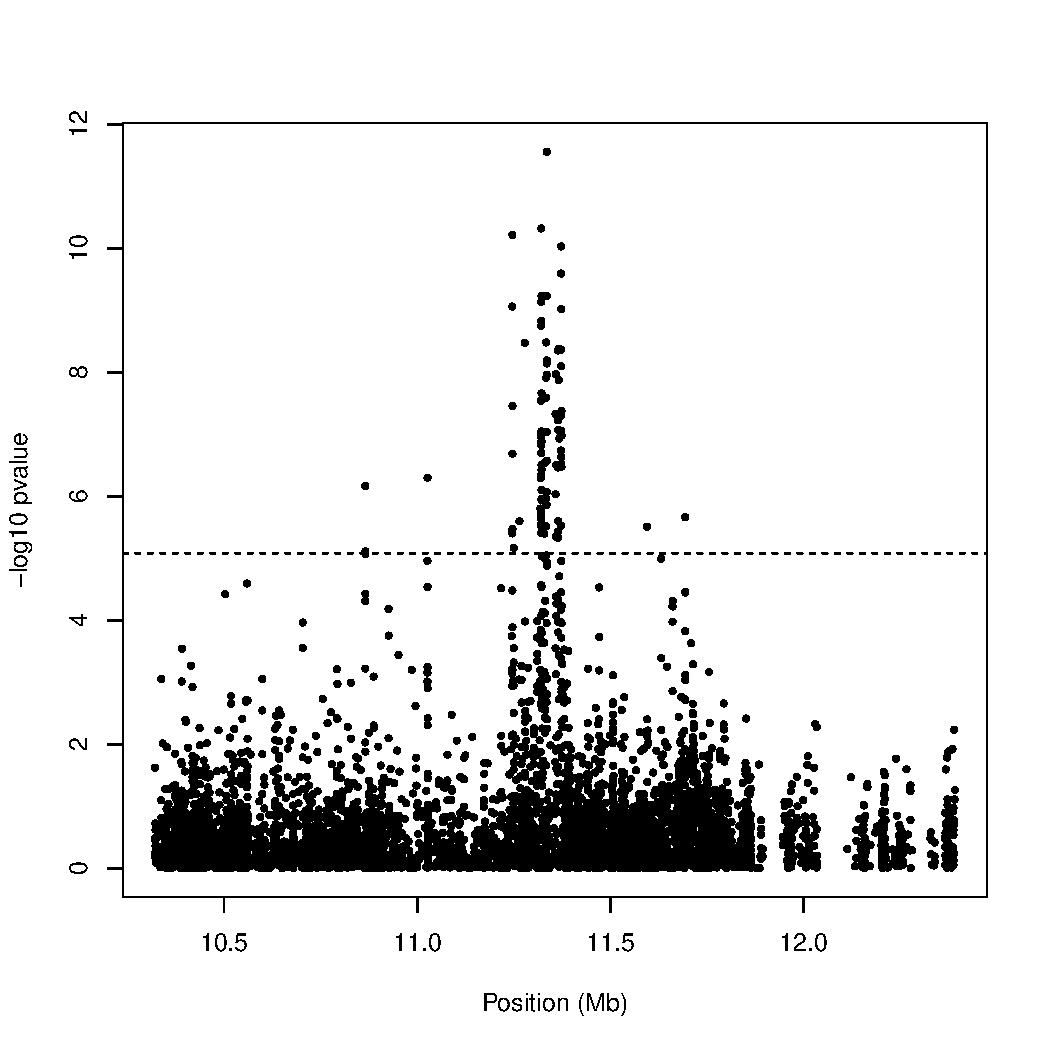
\includegraphics[width=\maxwidth]{figure/manPlot-1} 

\end{knitrout}

\begin{knitrout}
\definecolor{shadecolor}{rgb}{0.969, 0.969, 0.969}\color{fgcolor}\begin{kframe}
\begin{alltt}
\hlcom{# Break the region into sub-regions}
\hlstd{cl} \hlkwb{<-} \hlstd{bumphunter}\hlopt{::}\hlkwd{clusterMaker}\hlstd{(}\hlkwc{chr}\hlstd{=position}\hlopt{$}\hlstd{Chr,}
                               \hlkwc{pos}\hlstd{=position}\hlopt{$}\hlstd{Pos,}
                               \hlkwc{assumeSorted}\hlstd{=}\hlnum{TRUE}\hlstd{,}
                               \hlkwc{maxGap} \hlstd{=} \hlnum{500}\hlstd{)}
\end{alltt}


{\ttfamily\noindent\itshape\color{messagecolor}{\#\# Creating a generic function for 'nchar' from package 'base' in package 'S4Vectors'}}\begin{alltt}
\hlcom{# Some blocks are too big... put limit at 30}
\hlstd{index} \hlkwb{<-} \hlstd{cl}
\hlstd{maxInd} \hlkwb{<-} \hlkwd{max}\hlstd{(index)} \hlopt{+} \hlnum{1}

\hlstd{blockLengths} \hlkwb{<-} \hlkwd{table}\hlstd{(index)}
\hlkwa{while}\hlstd{(}\hlkwd{sum}\hlstd{(blockLengths} \hlopt{>} \hlnum{30}\hlstd{)} \hlopt{>} \hlnum{0}\hlstd{) \{}

  \hlkwa{for} \hlstd{(j} \hlkwa{in} \hlkwd{unique}\hlstd{(index)) \{}
    \hlstd{p} \hlkwb{<-} \hlkwd{length}\hlstd{(index[index} \hlopt{==} \hlstd{j])}
    \hlkwa{if} \hlstd{(p} \hlopt{>} \hlnum{30}\hlstd{) \{}
      \hlstd{q} \hlkwb{<-} \hlkwd{floor}\hlstd{(p}\hlopt{/}\hlnum{2}\hlstd{); r} \hlkwb{<-} \hlstd{p} \hlopt{-} \hlstd{q}
      \hlstd{index[index} \hlopt{==} \hlstd{j]} \hlkwb{<-} \hlkwd{c}\hlstd{(}\hlkwd{rep_len}\hlstd{(maxInd, q),}
                             \hlkwd{rep_len}\hlstd{(maxInd} \hlopt{+} \hlnum{1}\hlstd{, r))}
      \hlstd{maxInd} \hlkwb{<-} \hlstd{maxInd} \hlopt{+} \hlnum{2}
    \hlstd{\}}
  \hlstd{\}}
  \hlstd{blockLengths} \hlkwb{<-} \hlkwd{table}\hlstd{(index)}
\hlstd{\}}

\hlstd{cl} \hlkwb{<-} \hlstd{index}
\hlstd{index} \hlkwb{<-} \hlstd{cl}
\hlstd{counter} \hlkwb{<-} \hlnum{0}
\hlkwa{for}\hlstd{(j} \hlkwa{in} \hlkwd{sort}\hlstd{(}\hlkwd{unique}\hlstd{(cl))) \{}
  \hlstd{counter} \hlkwb{<-} \hlstd{counter} \hlopt{+} \hlnum{1}
  \hlstd{index[index} \hlopt{==} \hlstd{j]} \hlkwb{<-} \hlstd{counter}
\hlstd{\}}

\hlkwd{table}\hlstd{(}\hlkwd{table}\hlstd{(index))}
\end{alltt}
\begin{verbatim}
## 
##   1   2   3   4   5   6   7   8   9  10  11  12  13  14  15  16  17  18 
## 303 160  72  68  56  31  28  30  17  18  13   9  15   6  17  24  14  15 
##  19  20  21  22  23  24  25  26  27  28  29  30 
##  13  13   8   9   4   9   4   4   3   4   5   8
\end{verbatim}
\end{kframe}
\end{knitrout}

\begin{knitrout}
\definecolor{shadecolor}{rgb}{0.969, 0.969, 0.969}\color{fgcolor}\begin{kframe}
\begin{alltt}
\hlstd{pcev_out} \hlkwb{<-} \hlkwd{computePCEV}\hlstd{(methylation,} \hlkwc{covariate} \hlstd{= pheno,}
                        \hlkwc{estimation} \hlstd{=} \hlstr{"block"}\hlstd{,}
                        \hlkwc{inference} \hlstd{=} \hlstr{"permutation"}\hlstd{,}
                        \hlkwc{index} \hlstd{= index,} \hlkwc{nperm}\hlstd{=}\hlnum{10}\hlstd{)}
\end{alltt}
\end{kframe}
\end{knitrout}

\begin{knitrout}
\definecolor{shadecolor}{rgb}{0.969, 0.969, 0.969}\color{fgcolor}\begin{kframe}
\begin{alltt}
\hlcom{# Manhattan plot VIMP}
\hlstd{BLK_boundaries} \hlkwb{<-} \hlkwd{c}\hlstd{(}\hlnum{11235000}\hlstd{,} \hlnum{11385000}\hlstd{)}
\hlkwd{plot}\hlstd{(position}\hlopt{$}\hlstd{Pos}\hlopt{/}\hlnum{1e6}\hlstd{, pcev_out}\hlopt{$}\hlstd{VIMP,} \hlkwc{xlab}\hlstd{=}\hlstr{"Position (Mb)"}\hlstd{,}
     \hlkwc{ylab}\hlstd{=}\hlstr{"Variable Importance"}\hlstd{,} \hlkwc{pch}\hlstd{=}\hlnum{19}\hlstd{,} \hlkwc{cex}\hlstd{=}\hlnum{0.5}\hlstd{,} \hlkwc{ylim}\hlstd{=}\hlkwd{c}\hlstd{(}\hlnum{0}\hlstd{,}\hlnum{1}\hlstd{))}
\hlkwd{lines}\hlstd{(}\hlkwc{x}\hlstd{=BLK_boundaries}\hlopt{/}\hlnum{1e6}\hlstd{,} \hlkwc{y}\hlstd{=}\hlkwd{rep_len}\hlstd{(}\hlnum{0.9}\hlstd{,}\hlnum{2}\hlstd{),}\hlkwc{lwd}\hlstd{=}\hlnum{3}\hlstd{,} \hlkwc{col}\hlstd{=}\hlstr{'red'}\hlstd{)}
\end{alltt}
\end{kframe}
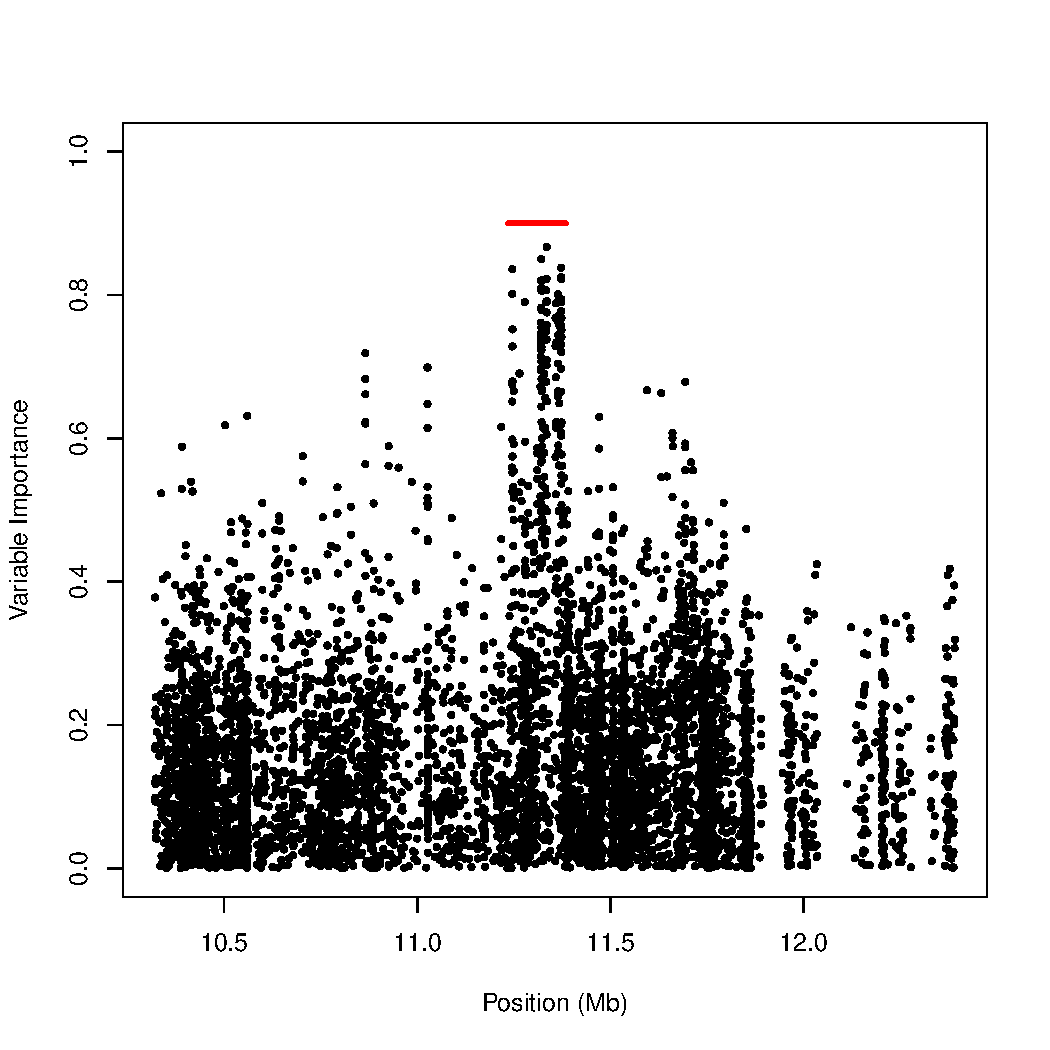
\includegraphics[width=\maxwidth]{figure/manPlotVIP-1} 

\end{knitrout}


\end{document}
